%%%%%%%%%%%%%%%%%%%%%%%%%%%%%%%%%%%%%%%%%%%%%%%%%%%%%%%%%%%%%%%
%
% Welcome to Overleaf --- just edit your LaTeX on the left,
% and we'll compile it for you on the right. If you open the
% 'Share' menu, you can invite other users to edit at the same
% time. See www.overleaf.com/learn for more info. Enjoy!
%
%%%%%%%%%%%%%%%%%%%%%%%%%%%%%%%%%%%%%%%%%%%%%%%%%%%%%%%%%%%%%%%
\documentclass{beamer}
\usetheme{Madrid}
\usecolortheme{seahorse}

\usepackage[linesnumbered,lined,boxed,commentsnumbered]{algorithm2e}

%%% Работа с русским языком и шрифтами
\usepackage[english,russian]{babel}   % загружает пакет многоязыковой вёрстки
% \usepackage{fontspec}      % подготавливает загрузку шрифтов Open Type, True Type и др.
% \setmainfont[Ligatures={TeX,Historic}]{Myriad Pro} 
% \setsansfont{Myriad Pro}  
% \setmonofont{Courier New}
\uselanguage{russian}
\languagepath{russian}
\deftranslation[to=russian]{Theorem}{Теорема}
\deftranslation[to=russian]{Definition}{Определение}
\deftranslation[to=russian]{Definitions}{Определения}
\deftranslation[to=russian]{Corollary}{Следствие}
\deftranslation[to=russian]{Fact}{Факт}
\deftranslation[to=russian]{Example}{Пример}
\deftranslation[to=russian]{Examples}{Примеры}

\graphicspath{{images/}} 

\let\eps\varepsilon
\let\tab\indent 
\let\inf\infty  % colision with infinum
\let\alp\alpha 

\newcommand{\expect}{\mathsf{E}}
\newcommand{\disp}{\mathsf{D}}

\newcommand{\N}{\mathbb{N}}
\newcommand{\Z}{\mathbb{Z}}
\newcommand{\R}{\mathbb{R}}
\newcommand{\CC}{\mathbb{C}}
\newcommand{\Q}{\mathbb{Q}}
\newcommand{\Real}{\mathrm{Re}}
\newcommand{\supp}{\mathrm{supp}}

\DeclareMathOperator{\im}{Im}
\DeclareMathOperator{\marg}{arg}
\DeclareMathOperator{\Arg}{Arg}

\DeclareMathOperator{\sign}{sgn}

\newcommand{\abs}[1]{\left|{#1}\right|}
\newcommand{\limit}[2][\infty]{\displaystyle{\lim_{{#2} \to {#1}}}\ }
\newcommand{\limitu}[1]{\displaystyle{\varlimsup_{{#1} \to \infty}}}
\newcommand*{\dlim}[2]{\underset{y \to #2}{\lim\limits_{x \to #1}}}
\newcommand{\mysum}[2]{\displaystyle{\sum^{#1}_{#2}}}
\newcommand{\answer}[1]{\\\fbox{Ответ: $\displaystyle{} {#1}$.}}
\newcommand{\Mod}[1]{\ \mathrm{mod}\ #1}
\newcommand{\seq}{\ \underset{\text{сх.}}{\sim} \ }

\newcommand{\bline}{ \noindent\makebox[\linewidth]{\rule{\paperwidth}{0.4pt}}}
\newcommand{\aliq}{\mathrel{\raisebox{-0.2ex}{\vdots}}}

\renewcommand{\d}[1]{\,d#1}
\newcommand{\prt}[2]{\frac{\partial{#1}}{\partial{#2}}}
\newcommand{\pprt}[2]{\frac{\partial^2{#1}}{\partial{#2}^2}}

\newenvironment{exercise}[2][Задача]{\begin{trivlist} 
\item[\hskip \labelsep {\bfseries #1}\hskip \labelsep {\bfseries #2.}]}{\end{trivlist}}

\everymath{\displaystyle}

\newcommand{\imp}[1]{\textit{\color{blue}#1}}

\newcommand{\uneq}[1]{\ \underset{#1}{=}\ }
\newcommand{\skipline}[0]{$ $\\}


\title{Графы в машинном обучении}
\author[Романов Владимир]{Романов Владимир БПМИ192}
\institute[ВШЭ]{Национальный исследовательский университет \\ «Высшая школа экономики» (Москва)}
\date{23 ноября 2021 г.}

\begin{document}

\frame{\titlepage}

\begin{frame}
    \frametitle{Какие задачи на графы нам интересны?}
    Задачи на вершины

    \begin{itemize}
        \item link-prediction
        \item node-classification
    \end{itemize}
    \skipline
    Задачи на графы

    \begin{itemize}
        \item graph-classification
    \end{itemize}
\end{frame}


\begin{frame}
    \frametitle{Vertex embeddings}
    Рассмотрим embedding, которые описывают локальные свойства
    \skipline
    \skipline
    Мы хотим, чтобы соседи имели близкий вектор, а далекие разный
    \skipline
    \skipline
    \skipline
    \skipline
    \pause
    Формулировка напоминает аналогичную задачу для текста
    \skipline
    \skipline
    \skipline
    \skipline
    Идея: попытаемся применить word2vec для этой задачи
\end{frame}

\begin{frame}
    \frametitle{DeepWalk (Постановка)}

    \begin{block}{Обозначения}
        Embedding: $\varPhi: V \to \R^d$ 
        \skipline
        \skipline
        Loss: $\sum_{\text{$u$ и $v$ <<близко>>}} -\ln \Prob\left(u \ \vert\ \varPhi(v)\right)$
    \end{block}
    \skipline
    \begin{block}{Алгоритм}
        \begin{enumerate}
            \item Переберем вершину $s \in V$
            \item Рассмотрим случайный путь $\mathcal{W}_s$ размера $t$
            \item Прорелаксируем SkipGram пройдясь по $\mathcal{W}_s$ окном $w$
            \item Повторим процес $\gamma$ раз
        \end{enumerate}
    \end{block}
\end{frame}

\begin{frame}
    \frametitle{DeepWalk (Hierarchical Softmax)}
    Проблема: SkipGram --- делать Softmax долго
    \skipline
    \skipline
    Решение: воспользуемся деревом отрезков
    \skipline
    % \skipline
    $ $\hspace*{4ex} 
    $
    \Prob\left(u \ \vert\ \varPhi(v)\right) = 
    \prod_{b_i \in B} \Prob\left(b_i \ \vert\ \varPhi(v)\right)
    $ 
    \skipline
    \skipline
    Итоговый алгоритм:
    \begin{figure}
        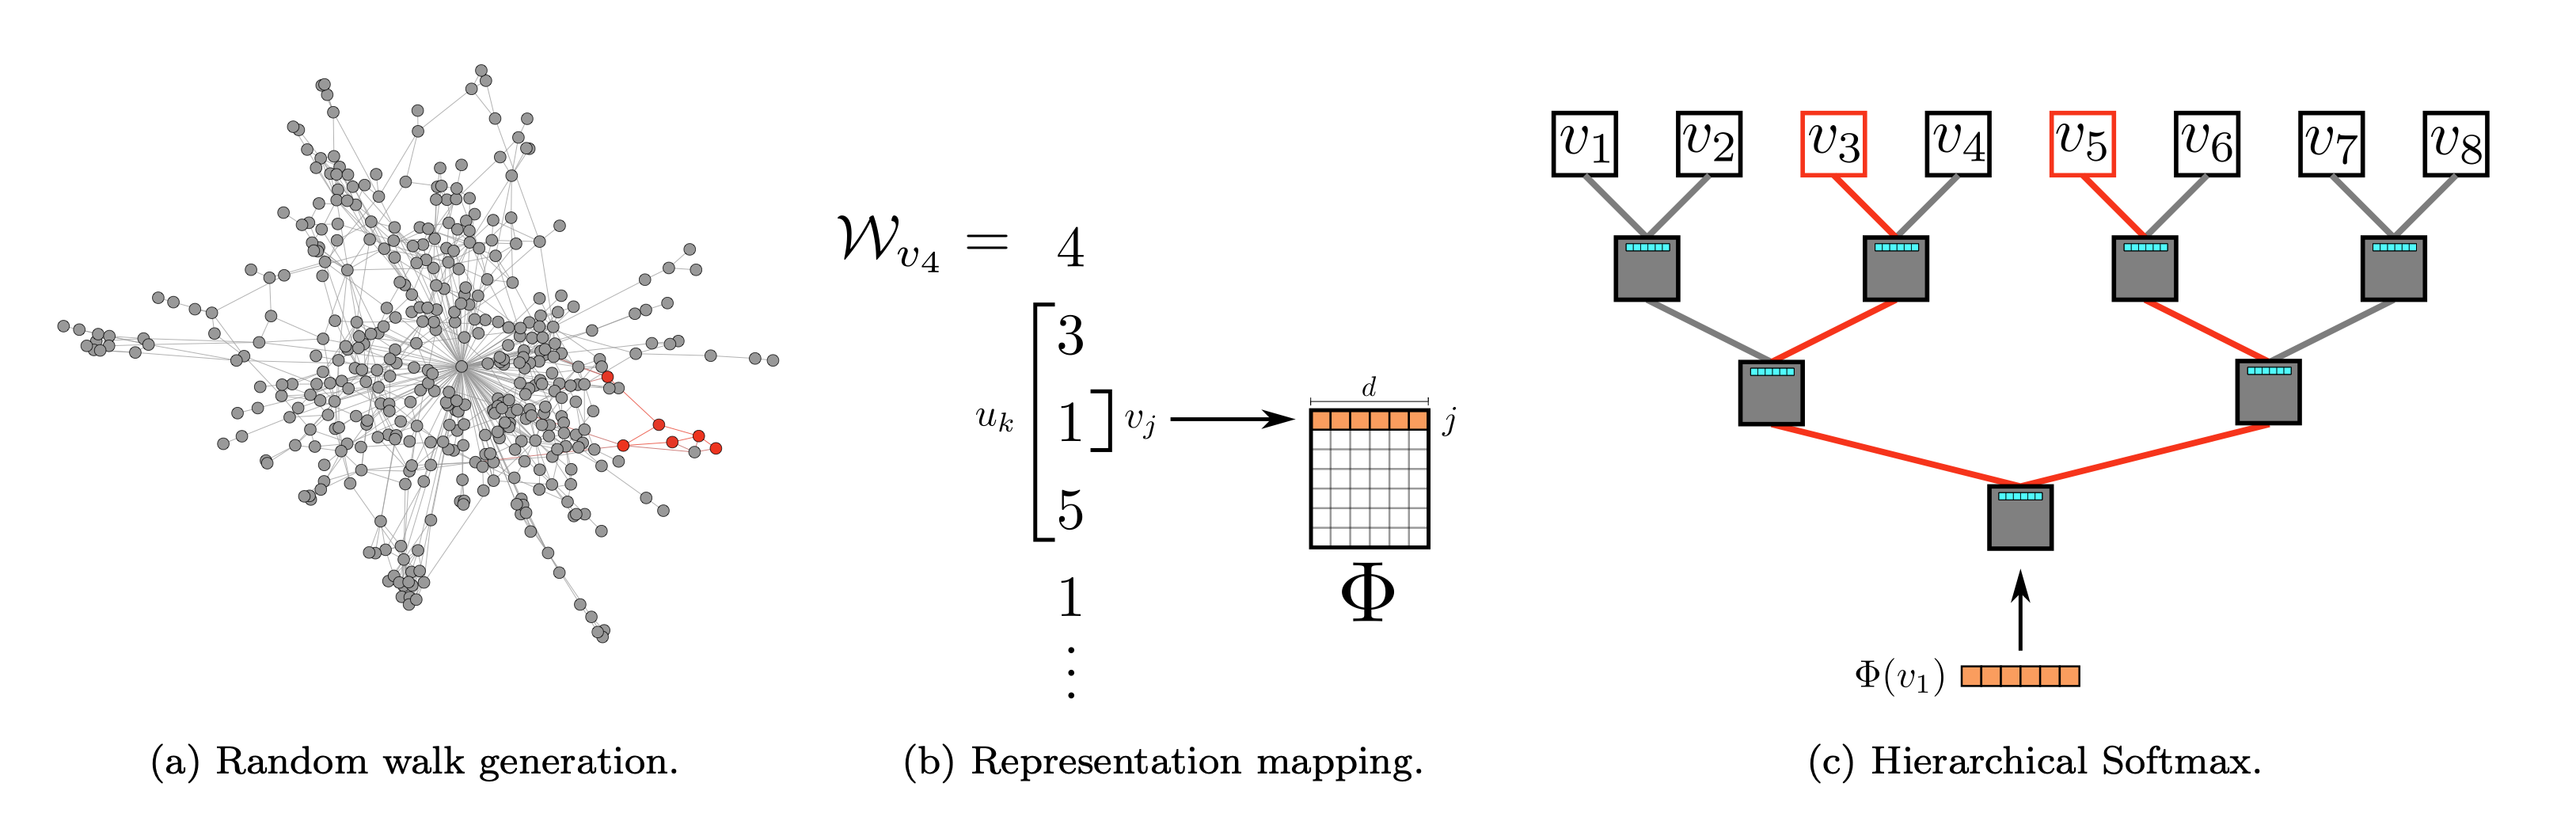
\includegraphics[width=1\columnwidth]{DeepWalk.png}
    \end{figure}
\end{frame}

\begin{frame}
\frametitle{Список литературы}
\begin{itemize}
    \item DeepWalk: \url{https://arxiv.org/pdf/1403.6652.pdf}
\end{itemize}
\end{frame}


\end{document}